\newpage
\phantomsection
\phantom{}
\thispagestyle{empty}
\addtocounter{page}{-1}
\newpage
\phantomsection
\phantom{}
\thispagestyle{empty}
\addtocounter{page}{-1}
\newpage
\phantomsection
\chapter*{Welcome!}


\phantom{}\vspace{7.7\baselineskip}

\noindent Copyright \copyright~2022 by Phillip Compeau. All rights reserved.\\

\noindent This book or any portion thereof may not be reproduced or used in any manner whatsoever without the express written permission of the publisher except for the use of brief quotations in a book review.\\

\noindent Printed in the United States of America\\

\noindent First Printing, 2022\\

\noindent ISBN: TBA\\

\noindent Library of Congress Control Number: TBA\\

\noindent Philomath Press, LLC
Pittsburgh, PA

%
%\thispagestyle{empty}
%
%
%
%\begin{dedication}
%\textit{To my family.}\hspace{0.98ex} --- P.\,C.\\[\baselineskip]
%\thispagestyle{empty}
%\end{dedication}
%
%\newpage \phantom{}
%\thispagestyle{empty}


% NEED TOC

\newpage



\nop{contents}{}
\tableofcontents*
\clearpage
\phantomsection

%Thank you for joining us!  Since its first publication in 2014, this textbook has become a bestseller in the field of computational biology, having been adopted by dozens of universities in twenty countries (\autopageref{sec:university_adoptions}).  Yet we are equally proud that the textbook also powers our popular online courses in bioinformatics, which have been completed by thousands of learners around the world.  We hope that you will sign up for our courses and explore our material online as well.
%
%You can also find lecture videos, PowerPoint slides, and answers to FAQs at the textbook website, \url{http://bioinformaticsalgorithms.org}.
%
%The subtitle of this book is \textit{An Active Learning Approach}.  This is because as you read, you will find a number of active learning components that will help you learn the material interactively and at your own pace.
%
%\begin{enumerate}
%\item \Black{Code Challenges} ask you to implement the algorithms that you will encounter (in any programming language you like).  These code challenges are hosted in the ``Bioinformatics Textbook Track'' location on Rosalind (\url{http://rosalind.info}), a website that will automatically test your implementations.  \marginpar{\centering\vskip-9ex\includegraphics[width = 3.6em]{images/CMYK_ed3/logos/rosalind}}
%\vspace{0.5\baselineskip}
%\item \Blue{Charging Stations} provide additional insights on implementing the algorithms you encounter.  However, we suggest trying to solve a Code Challenge before you visit a Charging Station.\marginpar{\centering\vskip-10.3ex{\includegraphics[width = 3.2em]{images/CMYK_ed3/logos/charging_station_intro}\\ \vskip-8.8ex }}
%%As one of our Coursera students once said, ``read, apply, fail the first attempt, then think carefully about the bigger picture as [you] try to understand why [your] first attempt failed.''
%\vspace{0.5\baselineskip}
%\item \Purple{\textbf{Exercise Breaks}} offer ``just in time'' assessments testing your understanding of a topic before moving to the next one.\marginpar{\centering\vskip-6.2ex\includegraphics[width = 3.2em]{images/CMYK_ed3/logos/exercise}}
%\vspace{0.5\baselineskip}
%\item \Red{STOP and Think} questions invite you to slow down and contemplate the current material before continuing to the next topic.\marginpar{\centering\vskip-6.1ex
\includegraphics[width = 3.2em]{images/CMYK_ed3/logos/stop_sign_no_border}}
%\vspace{0.5\baselineskip}
%\item \Orange{Detours} provide extra content that didn't quite fit in the main text.\nop{detour}\marginpar{\centering\vskip-3.3ex\hyperlink{detour}{\includegraphics[width = 6em]{images/CMYK_ed3/logos/detour_blank_no_bg_outline}\hskip-7em\vskip-4.9ex\parbox{7em}{\small\Black{~~~~\textsc{DETOUR}~}}}}
%\vspace{0.5\baselineskip}
%\item \Green{Challenge Problems} ask you to apply what you have learned to real experimental datasets.
%\item \Yellow{FAQs} \marginpar{\centering\vskip-4.6ex\includegraphics[width = 3.6em]{images/CMYK_ed3/logos/faq}} are questions that we encountered many times from the learners who have taken our online courses and the students we have taught using this book in our own offline courses.  When you see the question mark symbol in the margin, it indicates that there is an FAQ on the current subject; answers to FAQs are hosted at the textbook website.
%\end{enumerate}
%
%\noindent Finally, we have tried to make the book as fun to read as possible.  For example, since bioinformatics is still an ever-changing frontier, we decided to implement a Wild West theme for the book. Accordingly, you will notice that each chapter begins with a cartoon image showing the authors entangled in some adventure. What do these cartoons have to do with bioinformatics?  Continue reading to find out!

\newpage \phantomsection
\section{Meet the Team}
\label{section:meet_the_team}

\vspace{\baselineskip}

\parpic(20.55ex,25ex)[l][l]{\href{http://compeau.cbd.cmu.edu}{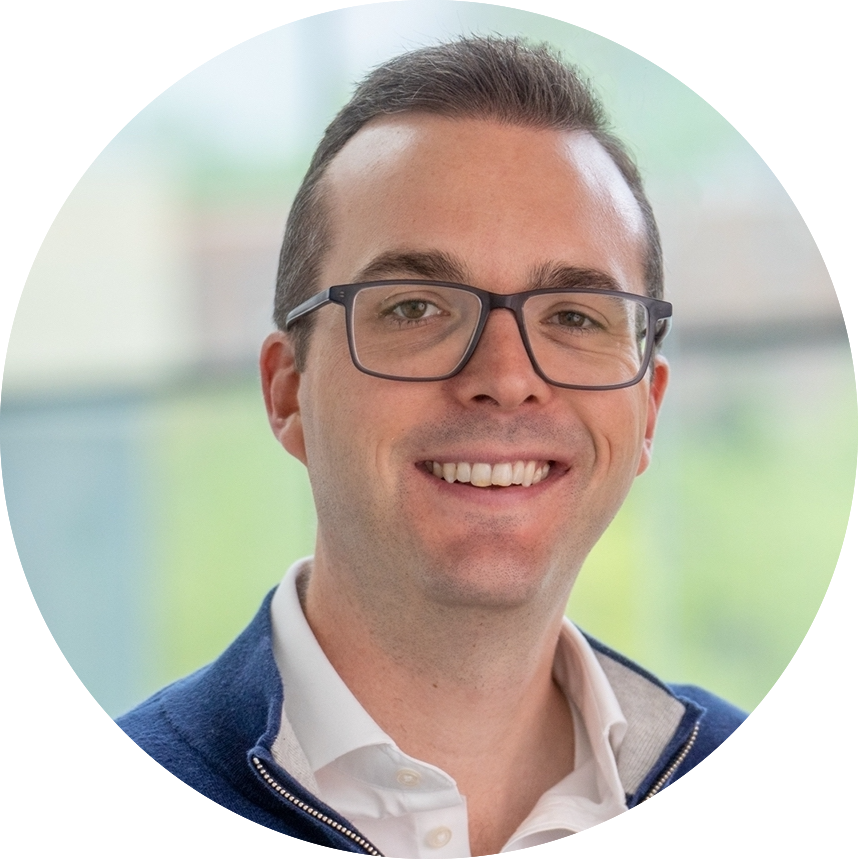
\includegraphics[width=19.26ex,clip,keepaspectratio]{../images/compeau_phillip_circle}}}
%\twitter[http://www.twitter.com/phillipcompeau]
%\linkedin[http://www.linkedin.com/in/phillipcompeau/]{0}
\vspace{0.2ex}\noindent {\small \href{http://compeau.cbd.cmu.edu}{\textbf{\textsc{Phillip Compeau}}} is the founder of \textit{Biological Modeling}. He is an Associate (Teaching) Professor and the Assistant Department Head in the Computational Biology Department at Carnegie Mellon University. He directs the undergraduate program in computational biology and co-directs the Precollege Program in Computational Biology, both of which he co-founded. He is passionate about open online education, and his education projects have reached hundreds of thousands of learners around the world. He is the co-author of \textit{Bioinformatics Algorithms: An Active Learning Approach}, which has been adopted by 200 instructors in 45 countries, and which powers the popular Bioinformatics Specialization on Coursera. He co-founded the learning platform Rosalind for learning programming, bioinformatics, and algorithms through independent problem solving, as well as the Programming for Lovers project, an online course in introductory programming motivated by fun scientific applications.}

\vspace{2.5\baselineskip}

\parpic(20.55ex, 26.97ex)[l][l]{\href{http://cseweb.ucsd.edu/~ppevzner/}{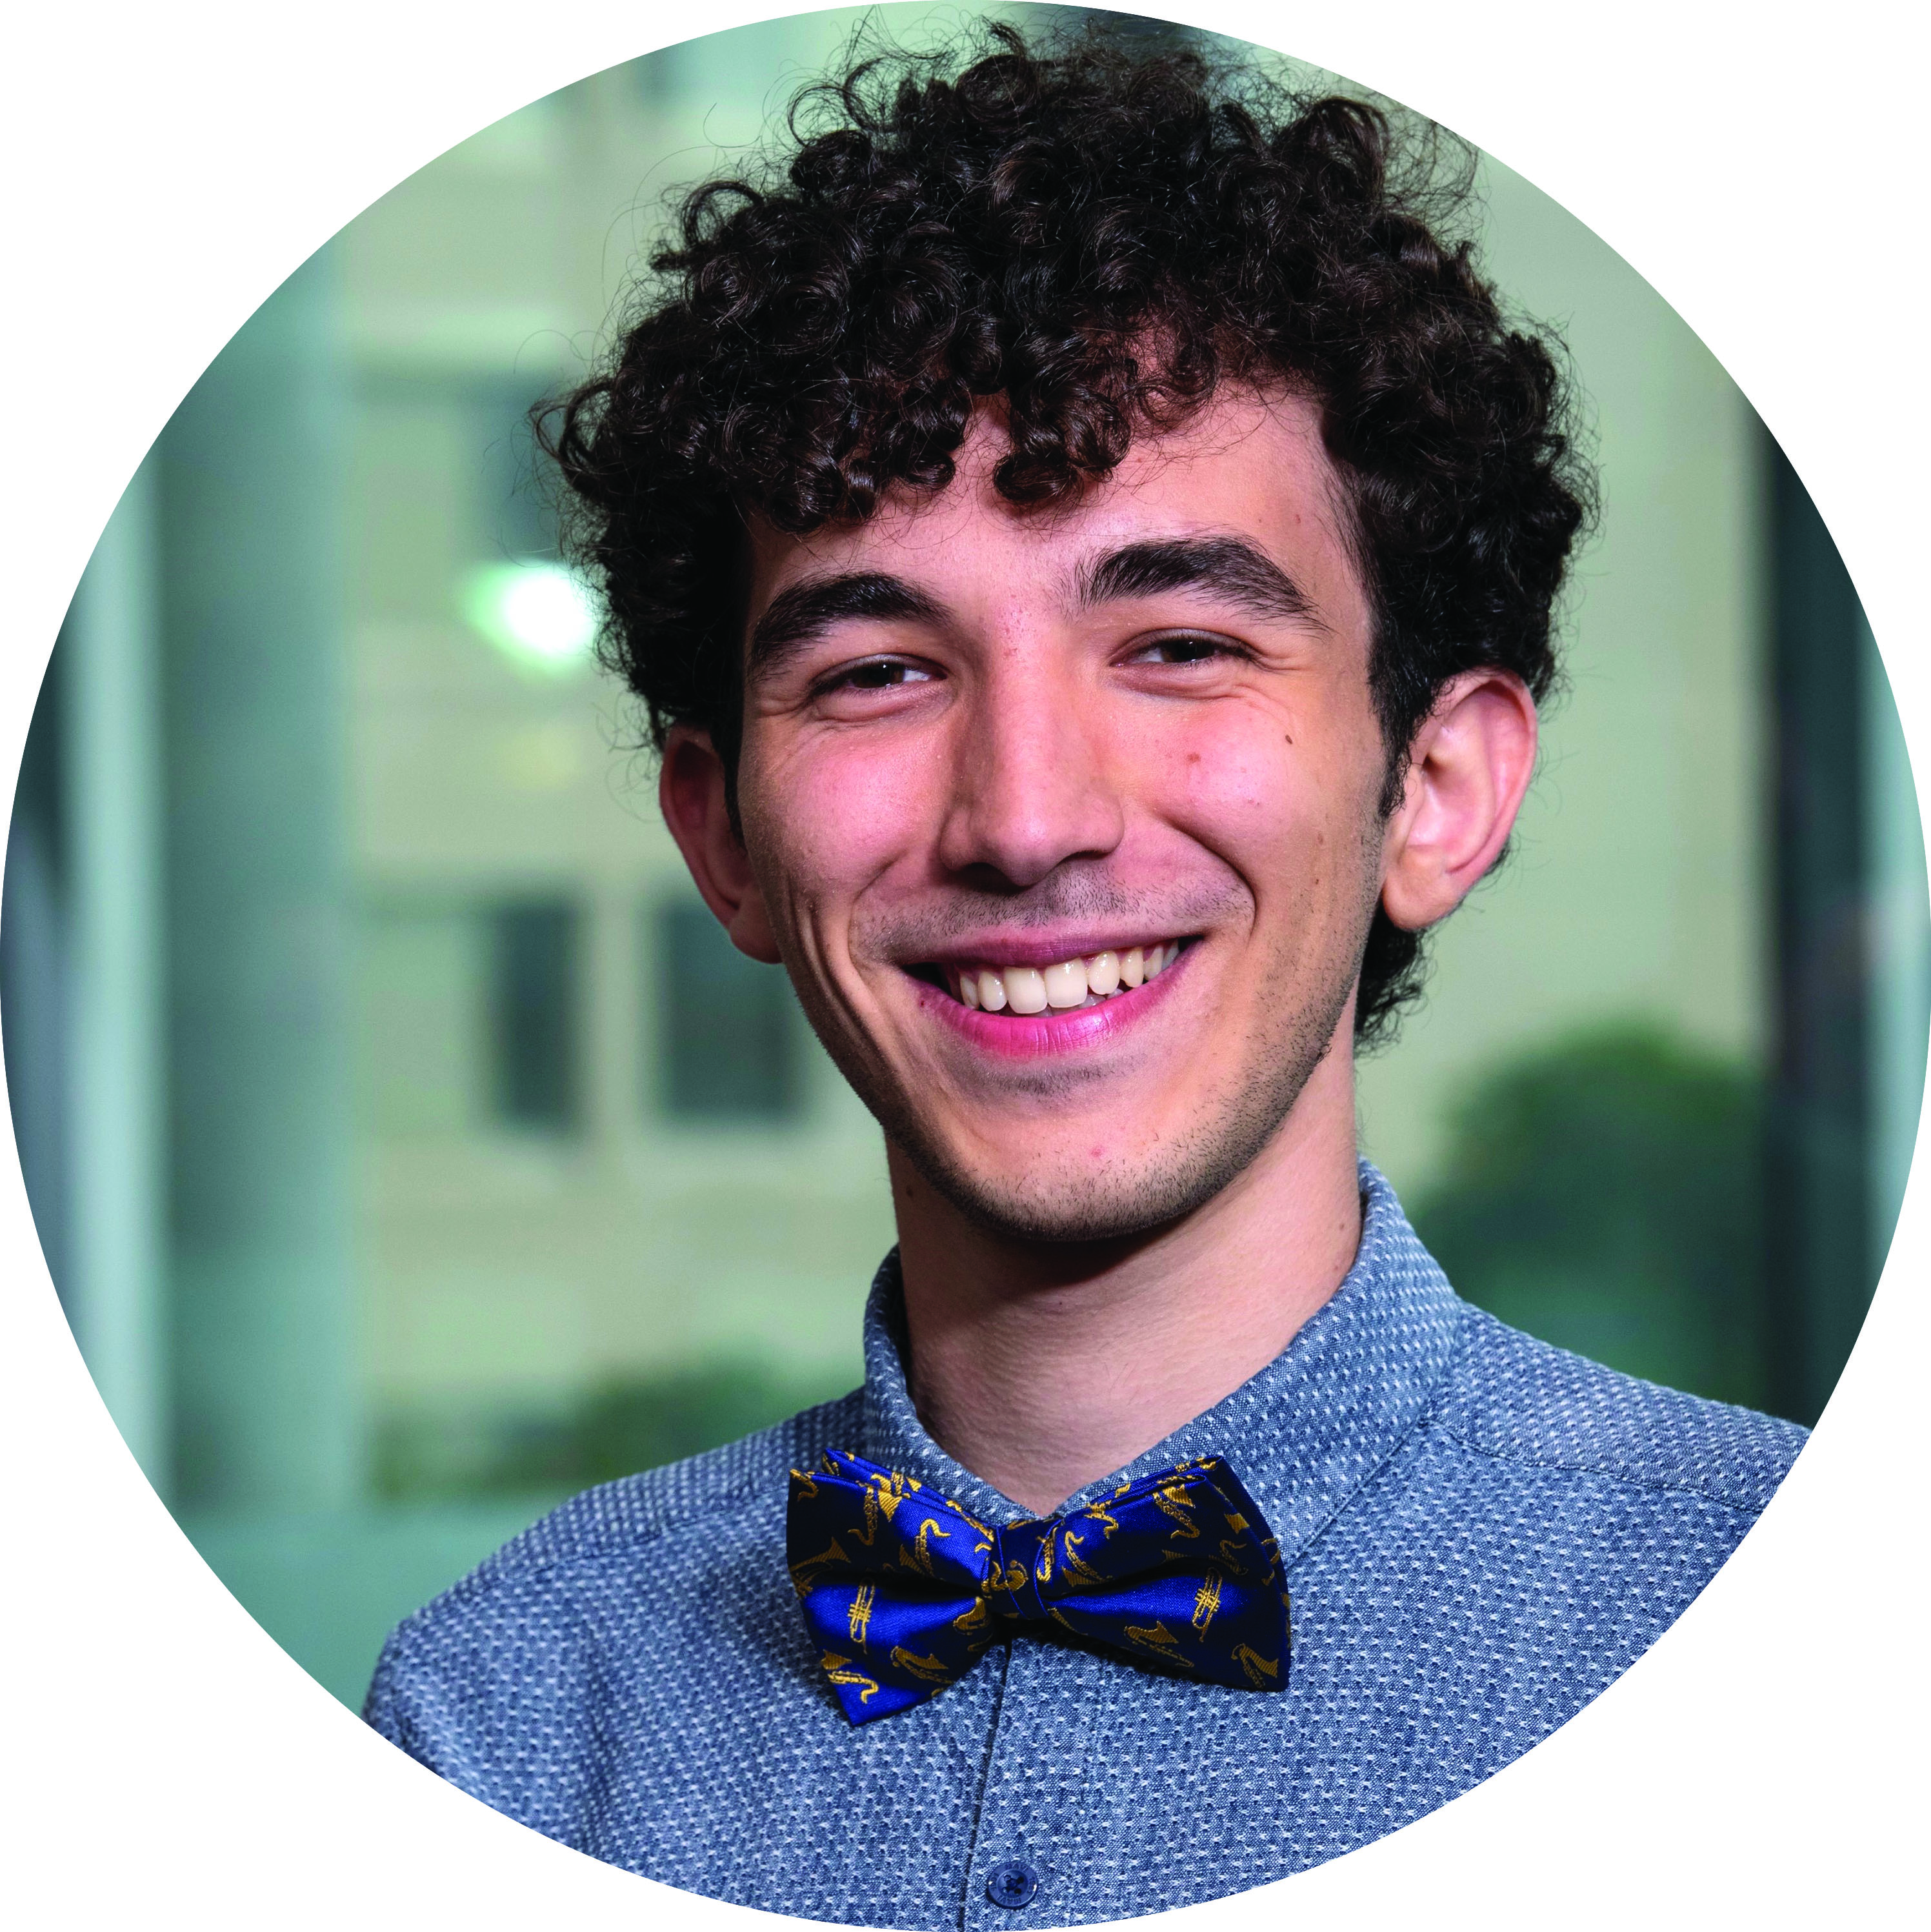
\includegraphics[width=19.26ex,clip,keepaspectratio]{../images/inan_mert_circle}}}
\vspace{0.85ex}\noindent {\small \textbf{\textsc{Mert Inan}} is a computer science Ph.D. student at the University of Pittsburgh. Mert is an alum of the M.S. in computational biology program at Carnegie Mellon University. He loves interdisciplinary fields and has been working at the intersection of computation, biology, neuroscience, and machine intelligence. Unlocking the secrets of biology is a pleasure that Mert truly enjoys, even under quarantine conditions.}

\vspace{2.5\baselineskip}

\parpic(20.55ex, 26.97ex)[l][l]{\href{http://cseweb.ucsd.edu/~ppevzner/}{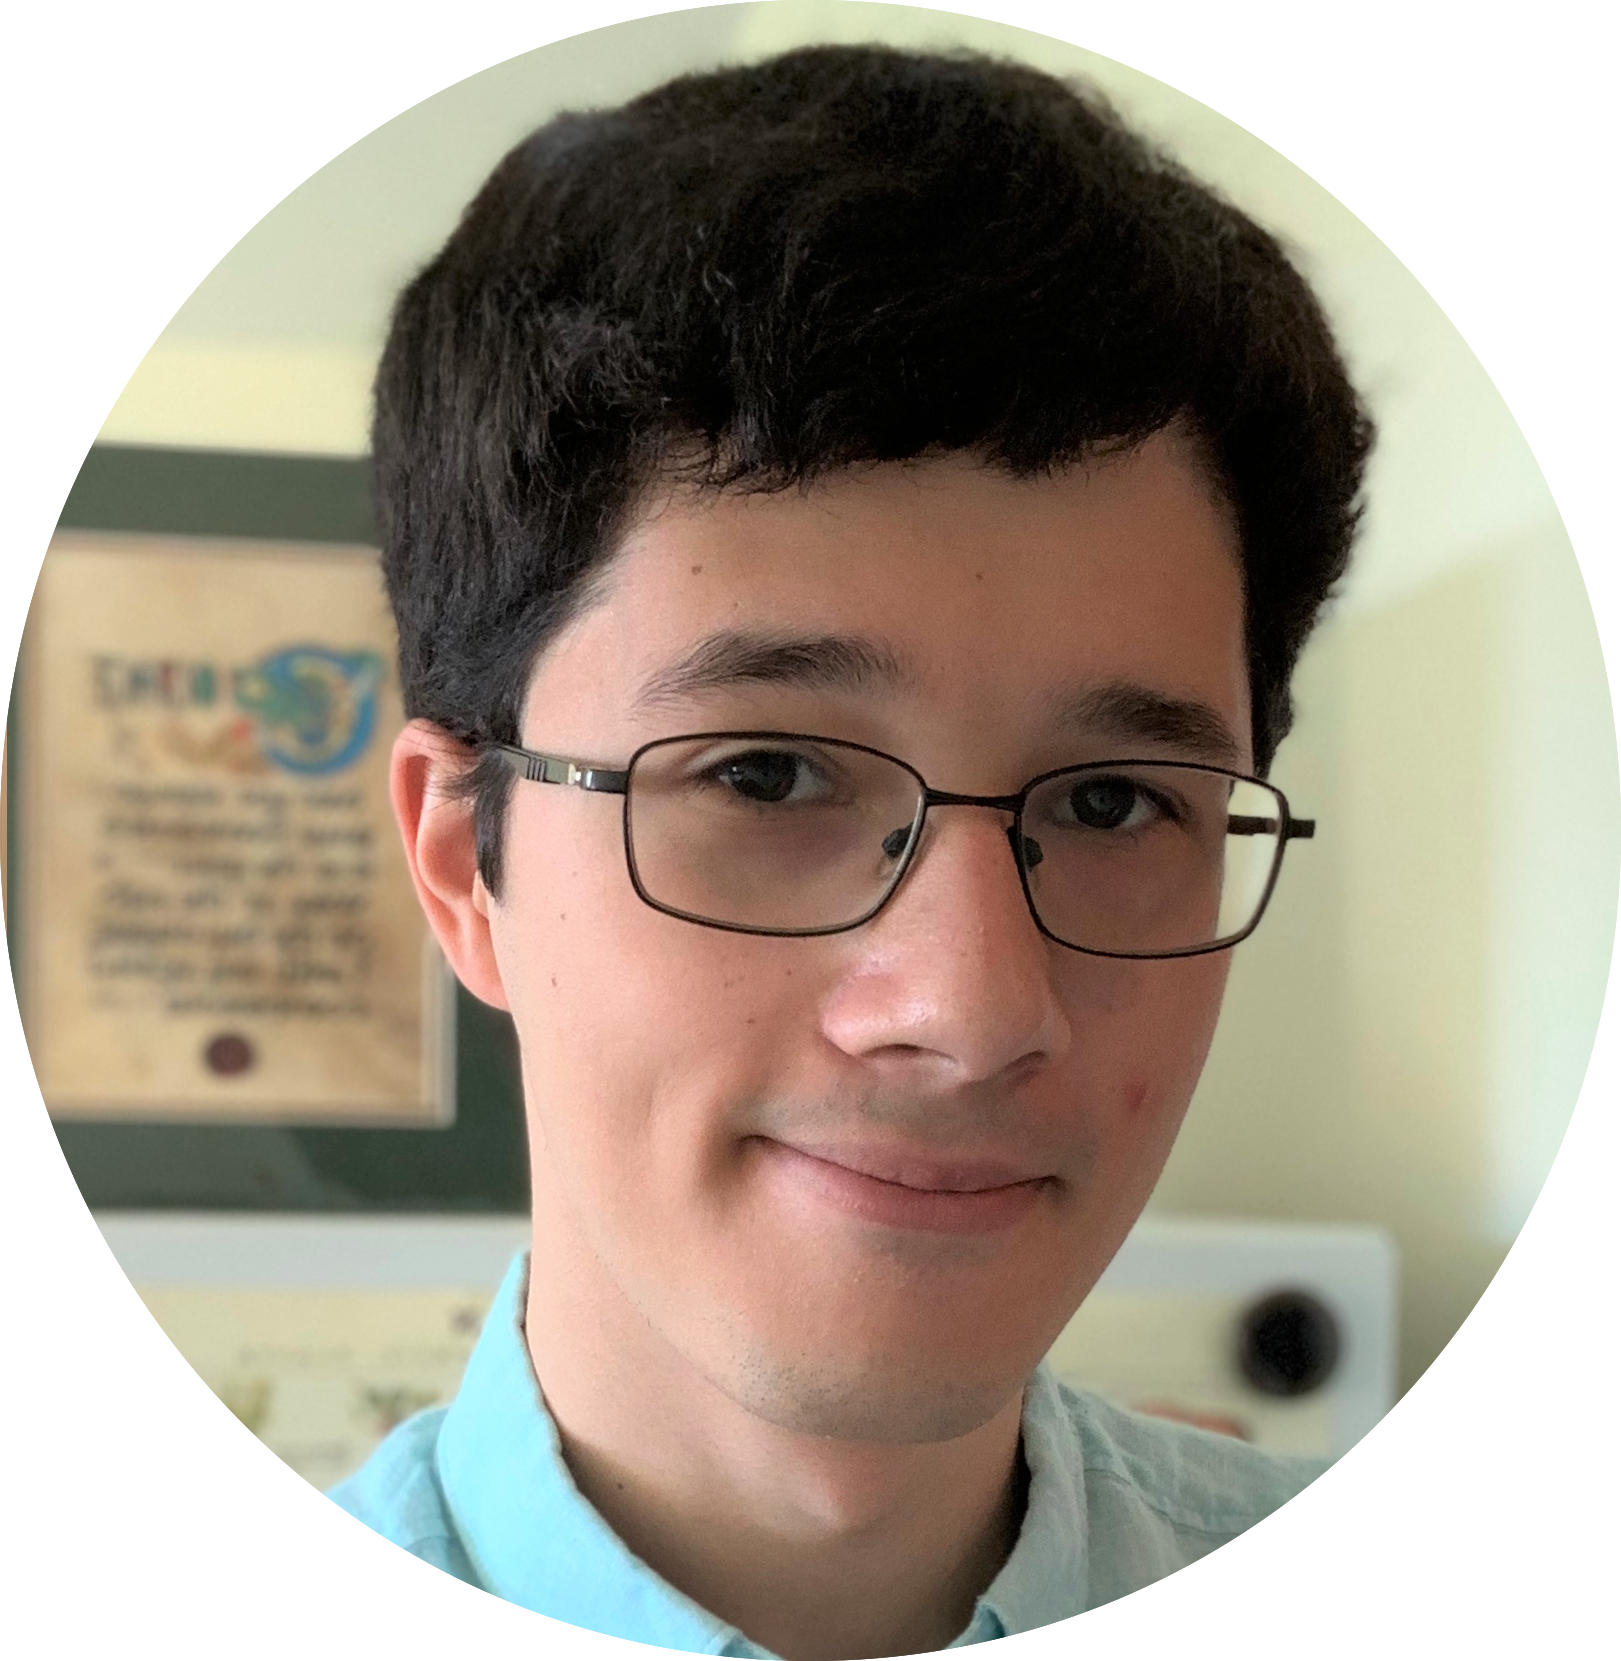
\includegraphics[width=19.26ex,clip,keepaspectratio]{../images/lee_noah_circle}}}
\vspace{0.85ex}\noindent {\small \textbf{\textsc{Noah Yann Lee}} is a PhD student at Yale University under the Computational Biology and Bioinfornatics program. Noah completed his undergraduate at Carnegie Mellon University, graduating in 2020 with a B.S. in Computational Biology with a minor in Design for Learning. From running early-childhood educational tests with the Children’s School at Carnegie Mellon for the Global Learning XPRIZE, to cultivating and sequencing phage genomes with the PhageHunters program, Noah has an appreciation for science from the micro to the macro, physical to the digital. Noah is always interested to connect with projects and organizations working with STEM, education, and science outreach.}

\vspace{2.5\baselineskip}

\parpic(20.55ex, 19.26ex)[l][l]{\href{http://cseweb.ucsd.edu/~ppevzner/}{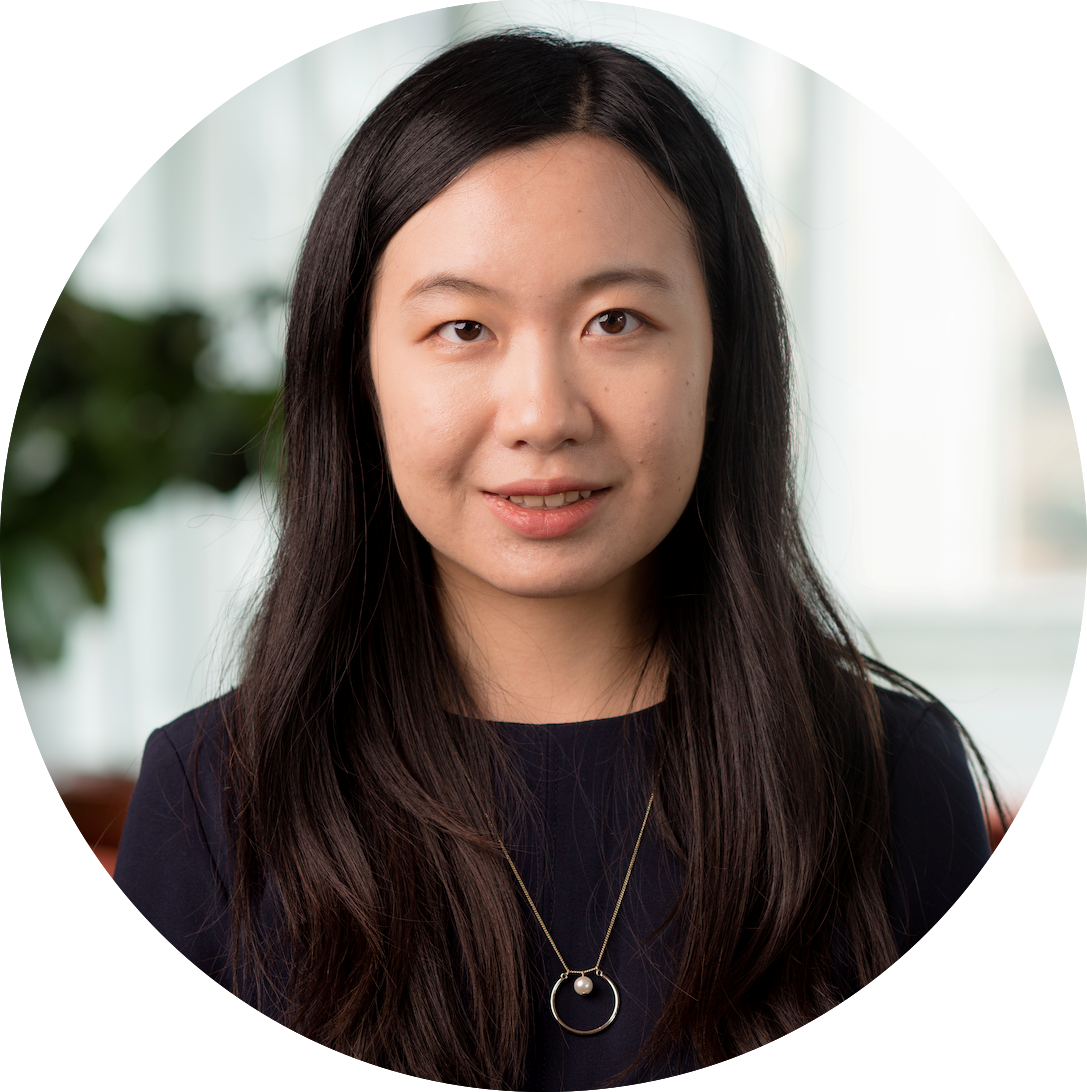
\includegraphics[width=19.26ex,clip,keepaspectratio]{../images/li_shuanger_circle}}}
\vspace{0.85ex}\noindent {\small \textbf{\textsc{Shuanger Li}} is a PhD student at the University of Chicago, and an alum of the M.S. in Computational Biology at Carnegie Mellon, where she worked with Dr. Oana Carja on heritable phenotypic variability. She enjoys modeling and simulation as powerful and fun ways to understand biological systems. She double majored in Environmental Sciences and Microbial Biology at UC Berkeley, where she studied Hawaiian arthropod assemblages, spider behaviors, and remediation bioreactors.}

\vspace{2.5\baselineskip}

\parpic(20.55ex, 19.26ex)[l][l]{\href{http://cseweb.ucsd.edu/~ppevzner/}{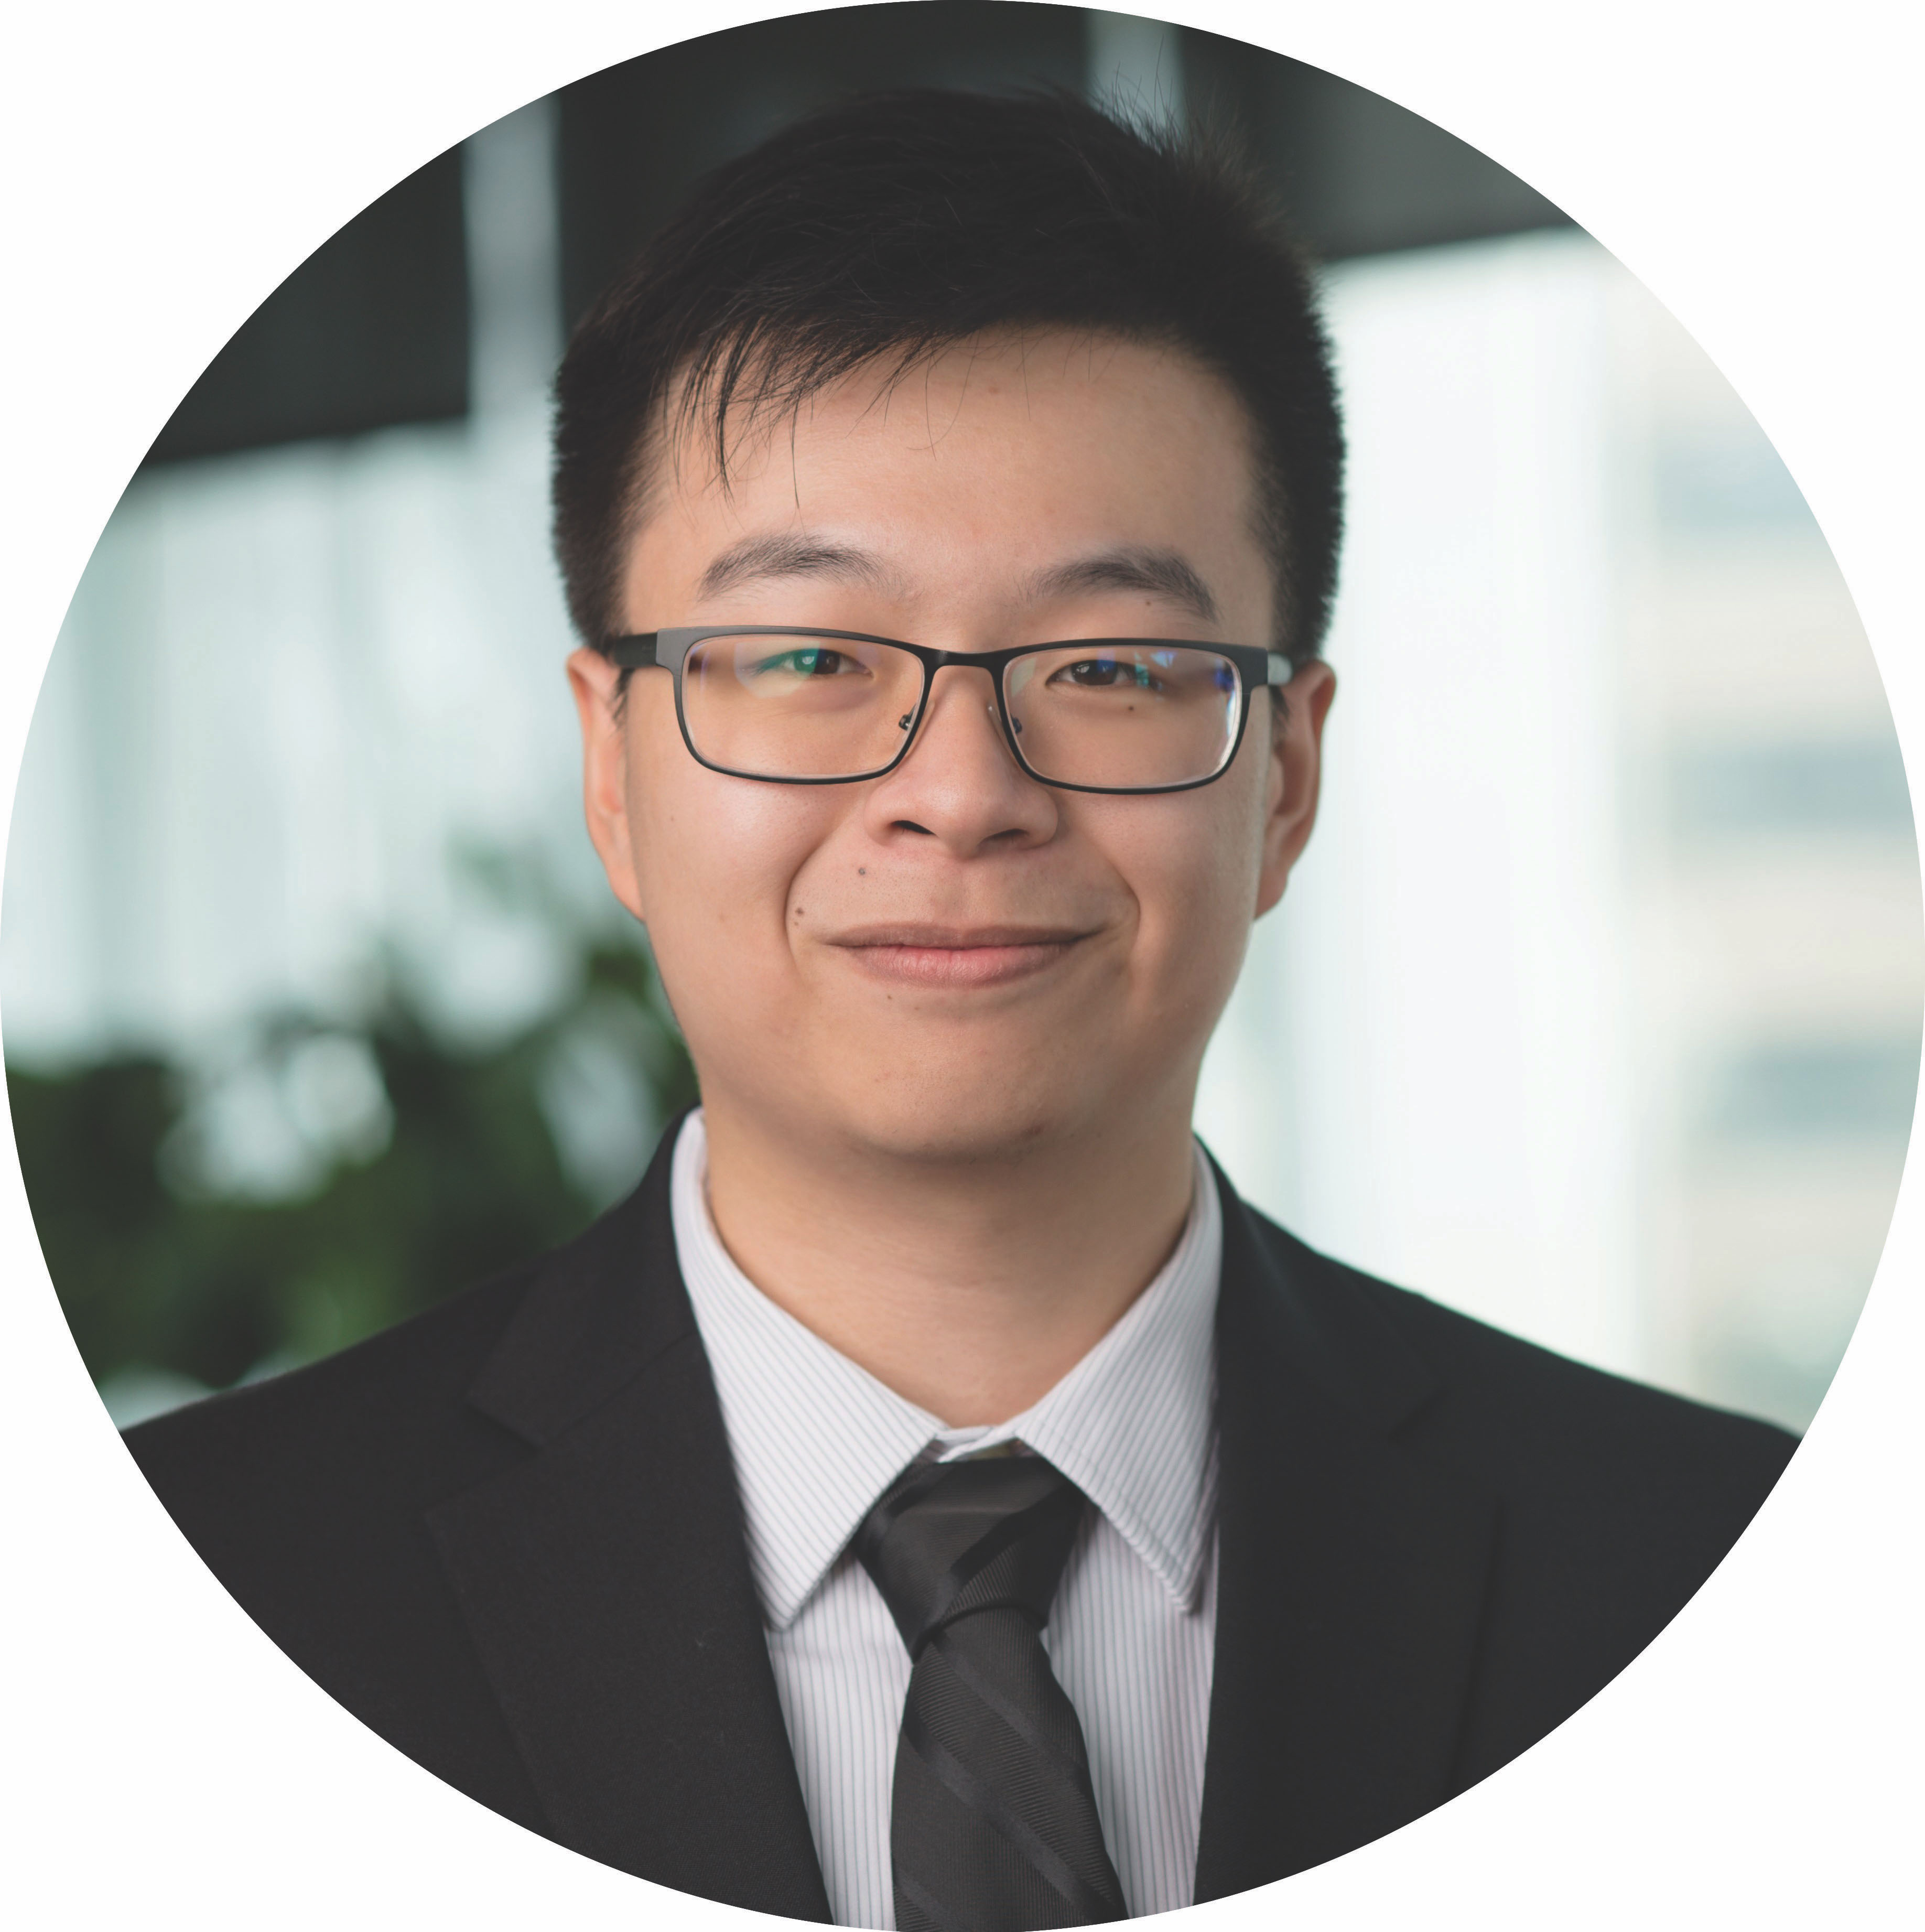
\includegraphics[width=19.26ex,clip,keepaspectratio]{../images/lee_chris_circle}}}
\vspace{0.85ex}\noindent {\small \textbf{\textsc{Chris Lee}} Chris Lee is an alum of the M.S. in Computational Biology at Carnegie Mellon University. Previously, he was an undergraduate student at Rutgers University and worked as an undergraduate researcher studying hydrothermal vent bacteria. In 2019, Chris graduated magna cum laude with a B.A. in Molecular Biology \& Biochemistry and double minor in Chemistry and Computer Science. He is currently interested in the fields of bioinformatics and genomics.}


 \clearpage
 \vspace{4.44ex}
 THIS PAGE IS A PLACEHOLDER BECAUSE OF BUGGY ISSUES WITH PARPIC.  DELETE IN FINAL VERSION, AS YOU CAN SEE \ldots THE PAGE IS NUMBERED THE SAME AS THE PREVIOUS PAGE\addtocounter{page}{-1}
 

 
\clearpage
\phantomsection
\chapter{Acknowledgments}
\label{chapter:acknowledgments}

God tier on Kickstarter
\begin{center}
\tabcolsep=2em
\begin{tabular}{l l}
Rumi Naik & Jill Gunn\\
Nicole Fontanese & Thomas Hutchinson Castro\\
Johnathon Nicolas Roman & Coralline Oz\\
Gillian Hawketts & Robert Lucyshyn\\
Ben Mescher & Jack and Will Haselhorst\\
Dave Lemen & Kevin Mai\\
Emily Tu & Othman Soufan\\
Suraj Nair & Joel Rodriguez Medina\\
Michael Li & Jason Dass\\
Austin Boucinha, OCT & Martin\\
Mark Mammel & Akash Ramachandran\\
Will Townes & Darrell Thomas\\
Sean Leonard & Eric Song\\
Hal Snyder & Jared A.~Davis\\
Kevin Reed & Iridium66\\
Maxwell Shapiro & Jérémie Sartor\\
Jeff Buck & Christopher James Langmead\\
Jacqueline McVeigh & Nikolett Lehel Lassie\\
Kelly Johnson & Jonathan McMenamin-Balano\\
Sassy Momassy & Mary B.~Kennedy\\
William S Owen & HD Welker\\
Wayne Myers & Adam Mihalik\\
Luther Tweneboah Evans & Braden Kartchner\\
Christos Noutsos & Costel Radu\\
Michael Levy & Leeza Sergeeva\\
Genene Hayes & Steven Fines\\
Jonathan M. & Gary L.~Keyfauver, PhD\\
Avinash Seetharamaiah & Steve Ross\\
Laura Climer & Joshua Coleman\\
Jim Reesman & Defne Surujon\\
Nick Connors & Pavel Pevzner\\
\end{tabular}
\end{center}

%
%\noindent This textbook was greatly improved by the efforts of a large number of individuals, to whom we owe a debt of gratitude.
%
%The development team, as well as Laurence Bernstein, Ksenia Krasheninnikova, Max Shen, and Jeffrey Yuan, implemented coding challenges and exercises, rendered figures, helped typeset the text, and offered insightful feedback on the manuscript.
%
%Glenn Tesler provided thorough chapter reviews and even implemented some software to catch errors in the early version of the manuscript!
%
%Robin Betz, Petar Ivanov, James Jensen, and Yu Lin provided insightful comments on the manuscript in its early stages. David Robinson was kind enough to copy edit a few chapters and palliate our punctuation maladies.
%
%Randall Christopher brought to life our crazy ideas for illustrations throughout the book, including the chapter header cartoons and the textbook cover.
%
%Andrey Grigoriev and Max Alekseyev gave advice on the content of \autoref{chapter:replication} and \autoref{chapter:rearrangements}, respectively. Martin Tompa helped us develop the narrative in \autoref{chapter:motifs} by suggesting that we analyze latent tuberculosis infection.
%
%Nikolay Vyahhi led a team composed of Andrey Balandin, Artem Suschev, Aleksey Kladov, and Kirill Shikhanov, who worked hard to support an online, interactive version of this textbook used in our online courses on Coursera.
%
%Our students on Coursera, especially Mark Mammel, Isabel Lupiani, Erika Ram\'irez and Dmitry Kuzminov, found hundreds of typos in our preliminary manuscript.
%
%Mikhail Gelfand, Uri Keich, Hosein Mohimani, Son Pham, and Glenn Tesler advised us on some of the book's ``Open Problems'' and led Massive Open Online Research projects (MOORs) in the first session of our online course.
%
%The Big Data to Knowledge Program at the National Institutes of Health, as well as Howard Hughes Medical Institute and the Russian Ministry of Education and Science generously gave their support for the development of the online courses accompanying this textbook.  The Bioinformatics and Systems Biology Program and the Computer Science \& Engineering Department at the University of California, San Diego provided additional support.
%
%Finally, our families gracefully endured the many long days and nights that we spent poring over manuscripts over the last several years; they helped us preserve our sanity along the way.
%
%\vspace{\baselineskip}
%
%\begin{minipage}{\textwidth}
%\raggedleft\noindent\parbox{0.18\textwidth}{\raggedright\itshape P.\,C. and P.\,P.\\
%May 2018
%}
%\end{minipage}

\newpage \phantom{}
\thispagestyle{empty}